Data races in parallel programs lead to non-deterministic behavior of programs. Therefore, data races are termed as errors. When access to a shared variable is protected by a lock, there is a programmer intended race on the variable. The behavior of the program is non-deterministic if the programmer does not order the way in which tasks access this shared variable, but, this behavior is expected by the programmer. 

Programs with data races can have different computation graph structures based on the schedule of tasks in the runtime (i.e., different update orders may result in different control flow paths). Similarly, when shared memory accesses are protected using locks, different computation graph structures can be observed based on the order in which the tasks access the protected shared variable. To ensure that a program in which tasks have mutually exclusive access to some shared variable does not have any unintended race, all the computation graph structures that can result from different schedules over the protected shared variable access have to be enumerated and analyzed.

\begin{figure*}
  \begin{center}
    \mprset{flushleft}
    \begin{mathpar}
     \and
      \inferrule[Isolated]
                {
				  \mathrm{canIsolate(C)} = \mathit{true} \\
                  n^\prime = \mathrm{fresh}() \\
                  N = N \cup \{n^\prime\} \\
                  E = E \cup \{\tuple{n, n^\prime},  \tuple{\mathit{last},n^\prime}\}\\
                }
{C[\tuple{\ell^\prime,S[\textbf{isolated}~s],\vec{r_\delta}^\prime,\vec{r_\omega}^\prime,d^\prime, n, 0}, m] \rightarrow
                  C[\tuple{\ell^\prime,
				   S[s; \textbf{isolated-end}],\vec{r_\delta}^\prime,\vec{r_\omega}^\prime,d^\prime, n^\prime, 1}, m]
                }
\and
      \inferrule[Isolated-Nested]
                {\mathit{iso} > 0 \\
                  \mathit{iso}^\prime = \mathit{iso} + 1
                }
{C[\tuple{\ell^\prime,S[\textbf{isolated}~s],\vec{r_\delta}^\prime,\vec{r_\omega}^\prime,d^\prime, n, \mathit{iso}}, m] \rightarrow
                  C[\tuple{\ell^\prime,
				   S[s; \textbf{isolated-end}],\vec{r_\delta}^\prime,\vec{r_\omega}^\prime,d^\prime, n, \mathit{iso}^\prime}, m]
}
\and
      \inferrule[Isolated-End-Nested]
                {\mathit{iso} > 1 \\
                  \mathit{iso}^\prime = \mathit{iso} - 1
                }
{C[\tuple{\ell^\prime,S[\textbf{isolated-end}],\vec{r_\delta}^\prime,\vec{r_\omega}^\prime,d^\prime, n, \mathit{iso}}, m] \rightarrow
                  C[\tuple{\ell^\prime,
				   S[\textbf{skip}],\vec{r_\delta}^\prime,\vec{r_\omega}^\prime,d^\prime, n, \mathit{iso}^\prime}, m]
                }
\and
      \inferrule[Isolated-End]
                {
                  n^\prime = \mathrm{fresh()}\\
                  \mathit{last} = n \\
                  N = N \cup \{n^\prime\} \\
                  E = E \cup \{\tuple{n, n^\prime}\}
                }
{C[\tuple{\ell^\prime,S[\textbf{isolated-end}],\vec{r_\delta}^\prime,\vec{r_\omega}^\prime,d^\prime, n, 1}, m] \rightarrow
                  C[\tuple{\ell^\prime,
				   S[\textbf{skip}],\vec{r_\delta}^\prime,\vec{r_\omega}^\prime,d^\prime, n^\prime,0}, m]
                }

\end{mathpar}
  \end{center}
  \caption{The transition rules for isolated statements.}
  \label{fig:isol-semantics}
\end{figure*}

The task parallel language is extended to model mutual exclusion with a new statement: $\textbf{isolated}~s$. The statement performs $s$ in mutual exclusion of any other isolated statements. The semantics with how the computation graph is impacted is in \figref{fig:isol-semantics}. The isolation is accomplished by creating a new global variable \textit{last} to track the last node in the computation graph belonging to an isolated statement, by adding to the task context a counter initialized to zero to count the number of nested isolated contexts, and with a new keyword for the rewrite rules: \textbf{isolated-end}. 

Let $\mathrm{canIsolate}(C)$ be a function over configurations to Boolean that returns true for a configuration tree if all the task counters are 0; otherwise it returns false. If no other isolated statements are running, then the \textsc{Isolated} rule increments the task counter to indicate isolation and inserts after the isolated statement $\mathit{s}$ the new \textbf{isolated-end} keyword. The computation graph gets a new node to track accesses in the isolated statement with an appropriate edge from the previous node. A sequencing edge from $\mathit{last}$ is also added so the previous isolated statement happens before this new isolated statement. As a note, $\mathit{last}$ is initialized to an empty node when execution starts. The \textsc{Isolated-Nested} rule simply increments the counter if the task is already in isolation.

The \textsc{Isolated-End-Nested} rule processes the new \textbf{isolated-end} keyword and decrements the counter. When the counter reaches the outer-most isolated context, the \textsc{Isolated-End} rule creates a new node in the computation graph to denote the end of isolation, and it updates $\mathit{last}$ to properly sequence any future isolation.

On-the-fly data race detection is modified for programs with isolated regions. When \textsc{Await-done} fires, the runtime checks if the region contains any task containing \textbf{isolated} statements. If the region does not have any isolated-nodes, data race detection is run on the region and if the region is data race free, it is replaced with an equivalent master node. If the region contains isolated-nodes, the program execution proceeds normally (i.e., on-the-fly data race detection is not executed on the region).

\begin{algorithm}
\caption{Scheduling algorithm for Isolated blocks.} \label{algo:isolated}
\begin{algorithmic}[1]
  \Function{schedule}{$t$, $\mathtt{Regs}$, $\mathtt{Tasks}$}
  \State \texttt{loop}:\ ($\mathtt{Regs}$, $\mathtt{Tasks}$) $:=$ \texttt{run}($t$, $\mathtt{Regs}$, $\mathtt{Tasks}$)\label{loc:run}
  \State $s :=$ \texttt{status}($t$)
  \State $R :=$ \texttt{runnable}($\mathtt{Tasks}$)
  \If{ $s =$ ISOLATED}\label{loc:entry:isolated}
  \ForAll{$t_i \in R$}\label{loc:prsched}
  \State \texttt{schedule}($t_i$, $\mathtt{Regs}$, $\mathtt{Tasks}$)
  \EndFor
  \Else
  \State $t_i$ := \texttt{random}($R$)\label{loc:rand}
  \State \texttt{schedule}($t_i$, $\mathtt{Regs}$, $\mathtt{Tasks}$)
  \EndIf
  \EndFunction
\end{algorithmic}
\end{algorithm}

Algorithm \ref{algo:isolated} presents a scheduling algorithm to explore different computation graph structures in parallel programs with isolated blocks. This algorithm is adapted from the scheduling algorithm used for model checking HJ programs using permission regions \cite{mercer2015model}. The algorithm considers a simplified state of the program with $\mathtt{Regs}$ as the set of region variables that are shared among the tasks, $\mathtt{Tasks}$ is the set of tasks and $t$ is a task. $R$ is the set of runnable tasks. 

The algorithm implements sequential semantics where only a single task is running at any time, and that task runs until it completes or isolates at which time a scheduling choice is made. Sequential semantics can be used for computation graph creation since Lemma 1 proves that the creation of computation graph is independent of the schedule that was followed to create the graph in the absence of data-race. And \corref{cor:notdrf} shows that if a data-race exists, then it manifests on every schedule. 

Line 2 updates the region variables and pool of tasks by running task $t$ until it exits, or reaches an \textbf{isolated}-construct. The function \texttt{status} on Line 3 returns the status of the task $t$. On Line 4, the function \texttt{runnable} is used to obtain a list of all the tasks that can be run from the pool of all tasks. If the status of the currently running task $t$ becomes \textsc{isolated} (i.e., the task encounters an \textbf{isolated} construct), the task is blocked and all the tasks that are runnable are scheduled by the runtime. When the task exits, a task is randomly selected from the set of runnable tasks and scheduled by the runtime.

\begin{figure}
  \begin{center}
    \begin{lstlisting}[mathescape=true]
  proc main(var n : int)
  	n := 1;
  	post $r_1 \leftarrow p_1~n~\varepsilon~\{r_1\}~\{r_1\}~\lambda v. n := n + v$;
  	post $r_1 \leftarrow p_2~n~\varepsilon~\{r_1\}~\{r_1\}~\lambda v. n := n + v$;
  	await $r_1$
 proc $p_1$(var n : int)
 	isolated $\texttt{l}(r_1) := n + 1$
 proc $p_2$(var n : int)
	isolated if $(\texttt{l}(r_1) = n)$ then
	  	post $r_1 \leftarrow p_3~n~\varepsilon~\{r_1\}~\{r_1\}~\lambda v. n := n + v$;
	else
		$\texttt{l}(r_1) := n - 1$
 proc $p_3$(var n : int)
	$\texttt{l}(r_1) := n+2$
\end{lstlisting}
  \end{center}
  \caption{Parallel program with mutual exclusion.}
  \label{fig:hj-isolated}
\end{figure}

\begin{figure*}
  \centering
  \subfigure[$t_1$ runs before $t_2$.]{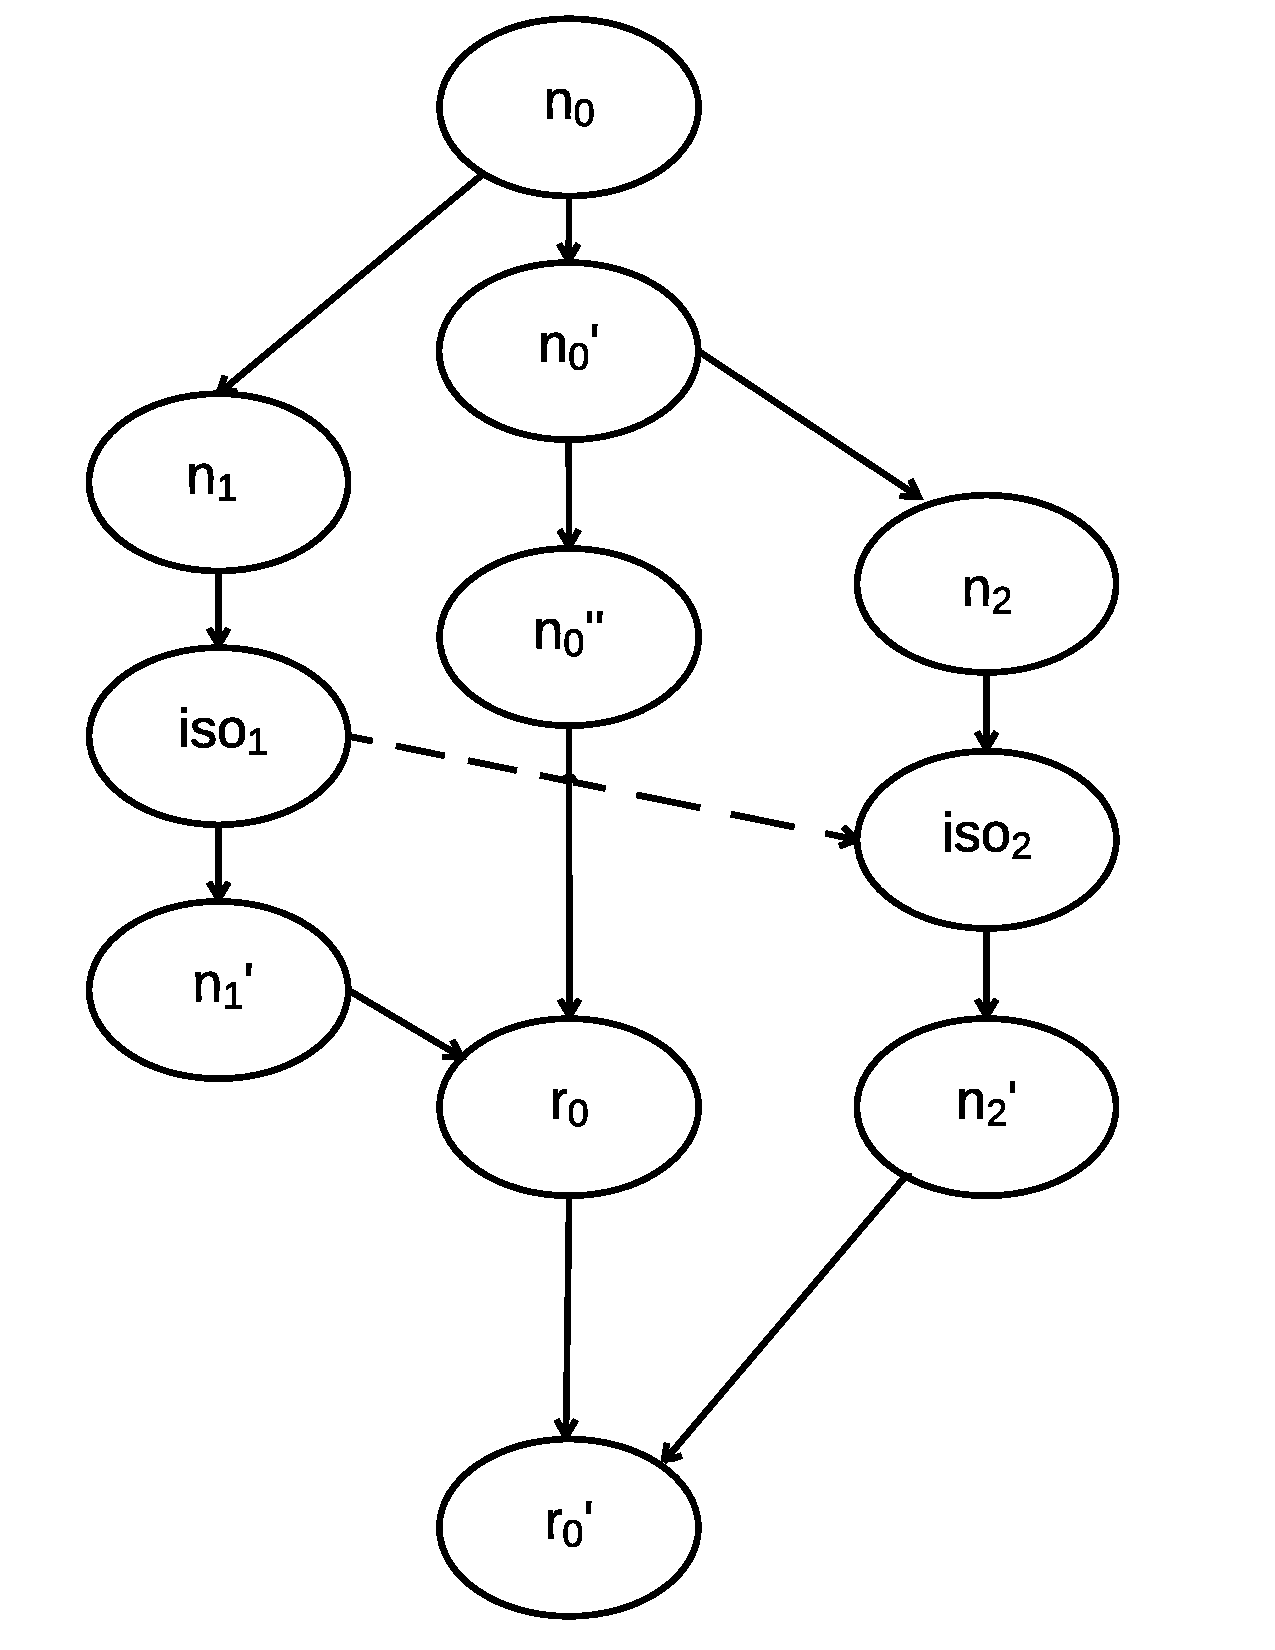
\includegraphics[scale=0.35]{../figs/Fig5-a.pdf}}
  \subfigure[$t_2$ runs before $t_1$.]{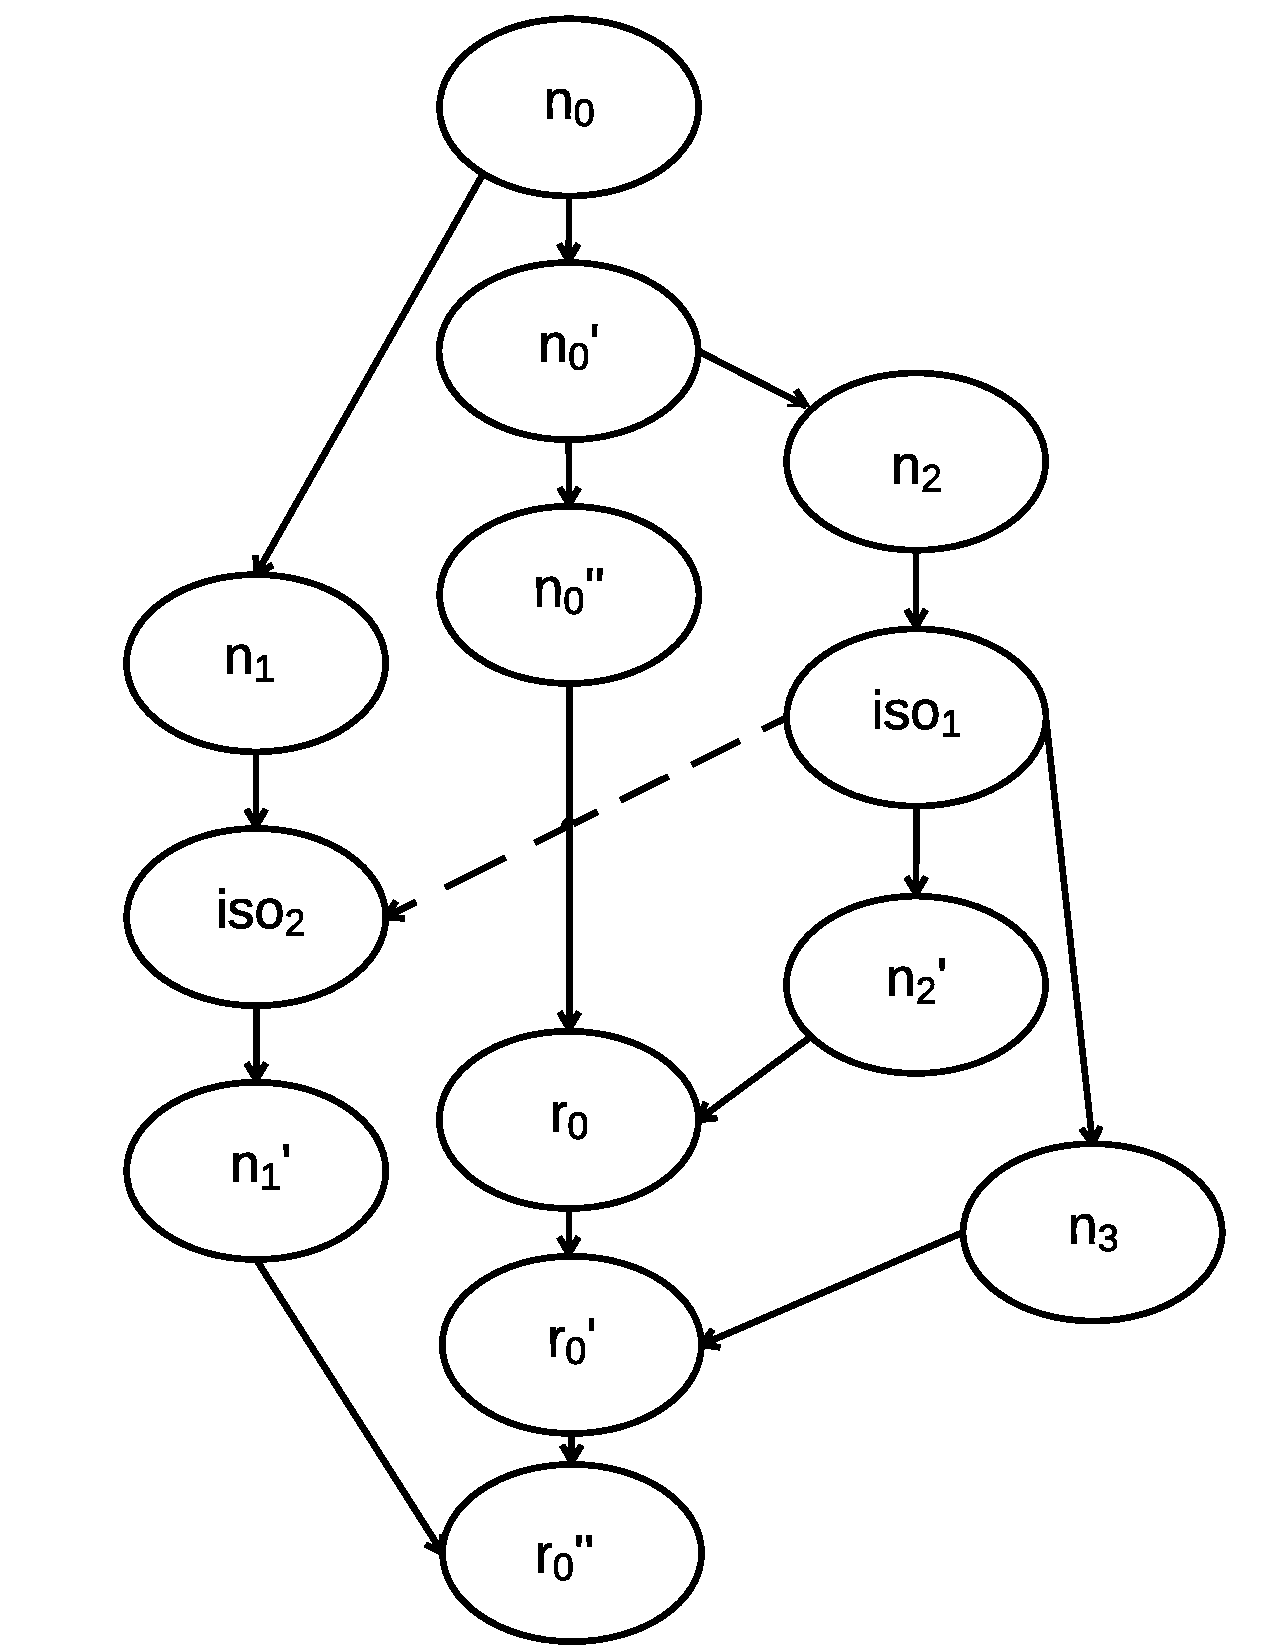
\includegraphics[scale=0.35]{../figs/Fig5-b.pdf}}
  \caption{Computation graphs of example in \figref{fig:hj-isolated}.}
   \label{fig:cg-isolated}
\end{figure*}

For the example in \figref{fig:hj-isolated}, two different computation graph structures can be formed based on the order of execution of isolated blocks. The computation graphs are shown in \figref{fig:cg-isolated}. If the scheduler runs the isolated section of task $t_1$ first, the computation graph in \figref{fig:cg-isolated}(a) is formed. Task $t_1$ changes the values of shared variable $r_1$ to 2. Hence, when task $t_2$ executes its isolated section, the if-condition fails and an additional task is not spawned by $t_2$. If the scheduler runs task $t_2$ first, the computation graph of \figref{fig:cg-isolated}(b) is formed. In this schedule, task $t_2$ executes its isolated section first. Since the value of variable $r_1$ is 1, the if-condition is met and a new task is created by $t_2$.

\begin{theorem}
Algorithm \ref{algo:isolated} finds all unique computation graphs for structured parallel programs with isolated sections making it sound and complete with Algorithm \ref{algo:drd}.
\end{theorem}

\begin{proof}
Theorem \ref{thm:strcutured-par-progs} states that Algorithm \ref{algo:drd} is sound and complete for structured parallel programs that do not contain isolated sections. If mutual exclusion is present, Algorithm \ref{algo:drd} does not remain sound since different computation graph structures can be formed for such programs. The different computation graph structures arise because the critical sections of tasks are executed in different orders under different program schedules. Algorithm \ref{algo:isolated} creates thread scheduling choices at the boundary of a critical section considering all the runnable threads that are present at the execution of a critical section. Hence, all relevant computation graphs are considered by \algoref{algo:drd}. Therefore, the data race detection using Algorithm \ref{algo:drd} becomes sound and complete when it is used along with Algorithm \ref{algo:isolated} for structured parallel programs that have mutual exclusion.
\end{proof}
